%% Default Latex document template
%%
%%  blake@rcs.ee.washington.edu

\documentclass[letterpaper]{article}

% Uncomment for bibliog.
%\bibliographystyle{unsrt}

\usepackage{graphicx}
\usepackage{lineno}
\usepackage{hyperref}
\usepackage{pdflscape}
%\usepackage{fancyhdr}

%%%%%%%%%%%%%%%%%%%%%%%%%%%%%%%%%%%%%%%%5
%
%  Set Up Margins

%%%%%%%%%%%%%%%%%%%%%%%%%%%%%%%%%%%%%%%%%%%%%%%%%
% include file for:
%      Critical Page setup dimensions
%            DO NOT MODIFY
%       (for help see "Latex Line by Line" p 260)
%
\setlength\oddsidemargin{0in}
\setlength\evensidemargin{0in}

\usepackage[left=0.98in, right=0.98in, top=1.0in, bottom=1.0in]{geometry}

% %Top Margin and header
% \setlength\voffset{-0.94in}
% \setlength\topmargin{0.25in}
% \setlength\headheight{0.25in}
% %\setlength\headwidth{6.5in}
% \setlength\headsep{0.25in}
% %Body
% \setlength\textwidth{6.5in}
% \setlength\textheight{9.50in}
% %Footer
% %\setlength\footheight{0.5in}
% \setlength\footskip{0.3750in}
% Line spacing for 6 lines per inch
\linespread{0.894}  % 1.0 = single    1.6 = double
%
%          END of Critical Page Setup Dimensions
%%%%%%%%%%%%%%%%%%%%%%%%%%%%%%%%%%%%%%%%%%%%%%%%%%%

%%%%%%%%%%%%%%%%%%%%%%%%%%%%%%%%%%%%%%%%%%%%%%%%%%%
%
% Useful style and math macros
%


\newcommand\Dfrac[2]{\frac{\displaystyle #1}{\displaystyle #2}}
\newcommand\beq{\begin{equation}}
\newcommand\eeq{\end{equation}}

\newcommand\bmat{\begin{bmatrix}}
\newcommand\emat{\end{bmatrix}}

\newenvironment{solution}
{\ttfamily \vspace{0.155in} {\bf SOLUTION:} \\ }
{ \vspace{0.25in} \par }



%
%        Font selection
%
%\renewcommand{\rmdefault}{ptm}             % Times
%\renewcommand{\rmdefault}{phv}             % Helvetica
%\renewcommand{\rmdefault}{pcr}             % Courier
%\renewcommand{\rmdefault}{pbk}             % Bookman
%\renewcommand{\rmdefault}{pag}             % Avant Garde
%\renewcommand{\rmdefault}{ppl}             % Palatino
%\renewcommand{\rmdefault}{pch}             % Charter


%%%%%%%%%%%%%%%%%%%%%%%%%%%%%%%%%%%%%%%%%%%%%%%%%
%
%         Page format Mods HERE
%
%Mod's to page size for this document
\addtolength\textwidth{0cm}
\addtolength\oddsidemargin{0cm}
\addtolength\headsep{0cm}
\addtolength\textheight{0cm}
%\linespread{0.894}   % 0.894 = 6 lines per inch, 1 = "single",  1.6 = "double"


% Make table rows deeper
%\renewcommand\arraystretch{2.0}% Vertical Row size, 1.0 is for standard spacing)

\begin{document}

\begin{center}
{\Large Simulation of Everting Tube Experiments: Data Supplement}\\
\end{center}

\section{Introduction}
The main document describes a two compartment model and parameter fitting procedure
for this type of eversion data.   In this supplement, we study the degree to which it
can fit all 9 eversion data sets despite qualitatively quite different behavior such
as smooth continuous eversion on some runs followed by discrete/jumpy eversion on others.

As described in Section XX of the main document, a structured parameter fitting procedure
was followed to fit all 9 datasets.   The starting point for all fits was an average of
all 9 parameter sets from previous fitting attempts.

\section{Dataset}

Lewis \cite{xxxxxxxx}  collected a set of nine eversion data as described in the main document.
Each data file contains, eversion length, derived eversion velocity, pressure (sensed within
tubing supplying the reservoir), and airflow (sensed near main air supply).   Tubes were loaded
with different values of supply reel inertia and supply reel Coulomb friction.  Three pieces
of tubing material were used multiple times to comprise the nine data sets.


\begin{landscape}
\section{Parameters}
After fitting each of the 9 datasets by following the model adjusting procedure, the parameters were
\begin{table}[!ht]
    \centering
    \begin{tabular}{|l|l|l|l|l|l|l|l|l|l|}
    \hline
        \textbf{Param Name} & \textbf{Set 0} & \textbf{Set 1} & \textbf{Set 2} & \textbf{Set 3} & \textbf{Set 4} & \textbf{Set 5} & \textbf{Set 6} & \textbf{Set 7} & \textbf{Set 8} \\ \hline
        \textbf{ET\_Res\_ratio} & 0.30 & 0.25 & 0.70 & 0.70 & 0.70 & 0.20 & 0.60 & 0.60 & 0.50 \\ \hline
        \textbf{K2drag} & 5.6 & 6.0 & 3.0 & 3.0 & 6.0 & 2.0 & 10.0 & -3.0 & -8.0 \\ \hline
        \textbf{Kdrag} & 2.11 & 1.00 & 0.50 & 0.50 & 4.00 & 0.80 & 6.50 & 3.00 & 8.00 \\ \hline
        \textbf{Lmax} & 0.70 & 0.43 & 0.70 & 0.70 & 0.55 & 0.45 & 0.55 & 0.55 & 0.54 \\ \hline
        \textbf{PBA\_static} & 118600 & 112000 & 112800 & 112800 & 112800 & 112000 & 105000 & 97500 & 105000 \\ \hline
        \textbf{PHalt\_dyn} & 116000 & 110000 & 111800 & 111800 & 111800 & 109800 & 108844 & 80000 & 100000 \\ \hline
        \textbf{Psource\_SIu} & 122020 & 117500 & 147000 & 147000 & 147000 & 120000 & 116000 & 116000 & 117000 \\ \hline
        \textbf{Rsource\_SIu} & 1.60E+08 & 1.30E+08 & 1.75E+08 & 1.75E+08 & 1.75E+08 & 1.40E+08 & 9.00E+07 & 9.00E+07 & 9.00E+07 \\ \hline
        \textbf{Tau\_coulomb} & 0.003222 & 0.002000 & 0.000200 & 0.000200 & 0.000200 & 0.002000 & 0.003222 & 0.003222 & 0.003222 \\ \hline
        \textbf{} & ~ & ~ & ~ & ~ & ~ & ~ & ~ & ~ & ~ \\ \hline
        \textbf{dt} & 0.000250 & 0.000250 & 0.000250 & 0.000250 & 0.000250 & 0.000250 & 0.000250 & 0.000250 & 0.000250 \\ \hline
        \textbf{et\_MPM} & 0.0032 & 0.0032 & 0.0032 & 0.0032 & 0.0032 & 0.0032 & 0.0032 & 0.0032 & 0.0032 \\ \hline
        \textbf{rReel} & 0.011 & 0.011 & 0.011 & 0.011 & 0.011 & 0.011 & 0.011 & 0.011 & 0.011 \\ \hline
        \textbf{Vhousing\_m3} & 0.00126 & 0.00126 & 0.00126 & 0.00126 & 0.00126 & 0.00126 & 0.00126 & 0.00126 & 0.00126 \\ \hline
        \textbf{Compartments} & 2 & 2 & 2 & 2 & 2 & 2 & 2 & 2 & 2 \\ \hline
        \textbf{COMP1} & supp\_tube & supp\_tube & supp\_tube & supp\_tube & supp\_tube & supp\_tube & supp\_tube & supp\_tube & supp\_tube \\ \hline
        \textbf{DataFile} & eb610645 & 15g42423 & 0ddc3bfa & 5d0f0862 & 4bf58872 & c4f507b1 & 891a0abc & e50137ee & 52f8bea7 \\ \hline
        \textbf{T} & 295.4 & 295.4 & 295.4 & 295.4 & 295.4 & 295.4 & 295.4 & 295.4 & 295.4 \\ \hline
        \textbf{RT} & 2456 & 2456 & 2456 & 2456 & 2456 & 2456 & 2456 & 2456 & 2456 \\ \hline
        \textbf{Patmosphere} & 101320 & 101320 & 101320 & 101320 & 101320 & 101320 & 101320 & 101320 & 101320 \\ \hline
        \textbf{ET\_Res\_per\_m} & 0.000120 & 0.000120 & 0.000120 & 0.000120 & 0.000120 & 0.000120 & 0.000120 & 0.000120 & 0.000120 \\ \hline
        \textbf{ET\_RofL\_mode} & constant & constant & constant & constant & constant & constant & constant & constant & constant \\ \hline
        \textbf{Threshold Taper} & 0.0 & 0.0 & 0.0 & 0.0 & 0.0 & 0.0 & 0.0 & 0.0 & 0.0 \\ \hline
    \end{tabular}
    \caption{Fitted parameters for the 9 data sets.}
\end{table}
\clearpage
\end{landscape}

\section{Simulations}

\section{Simulation Results: 8 everting tube experiments}
Each figure illustrates the results of the simulation and parameter tuning process described in the main paper, Section X.X.X.
\vspace{0.5in}

\begin{figure}[h]\centering
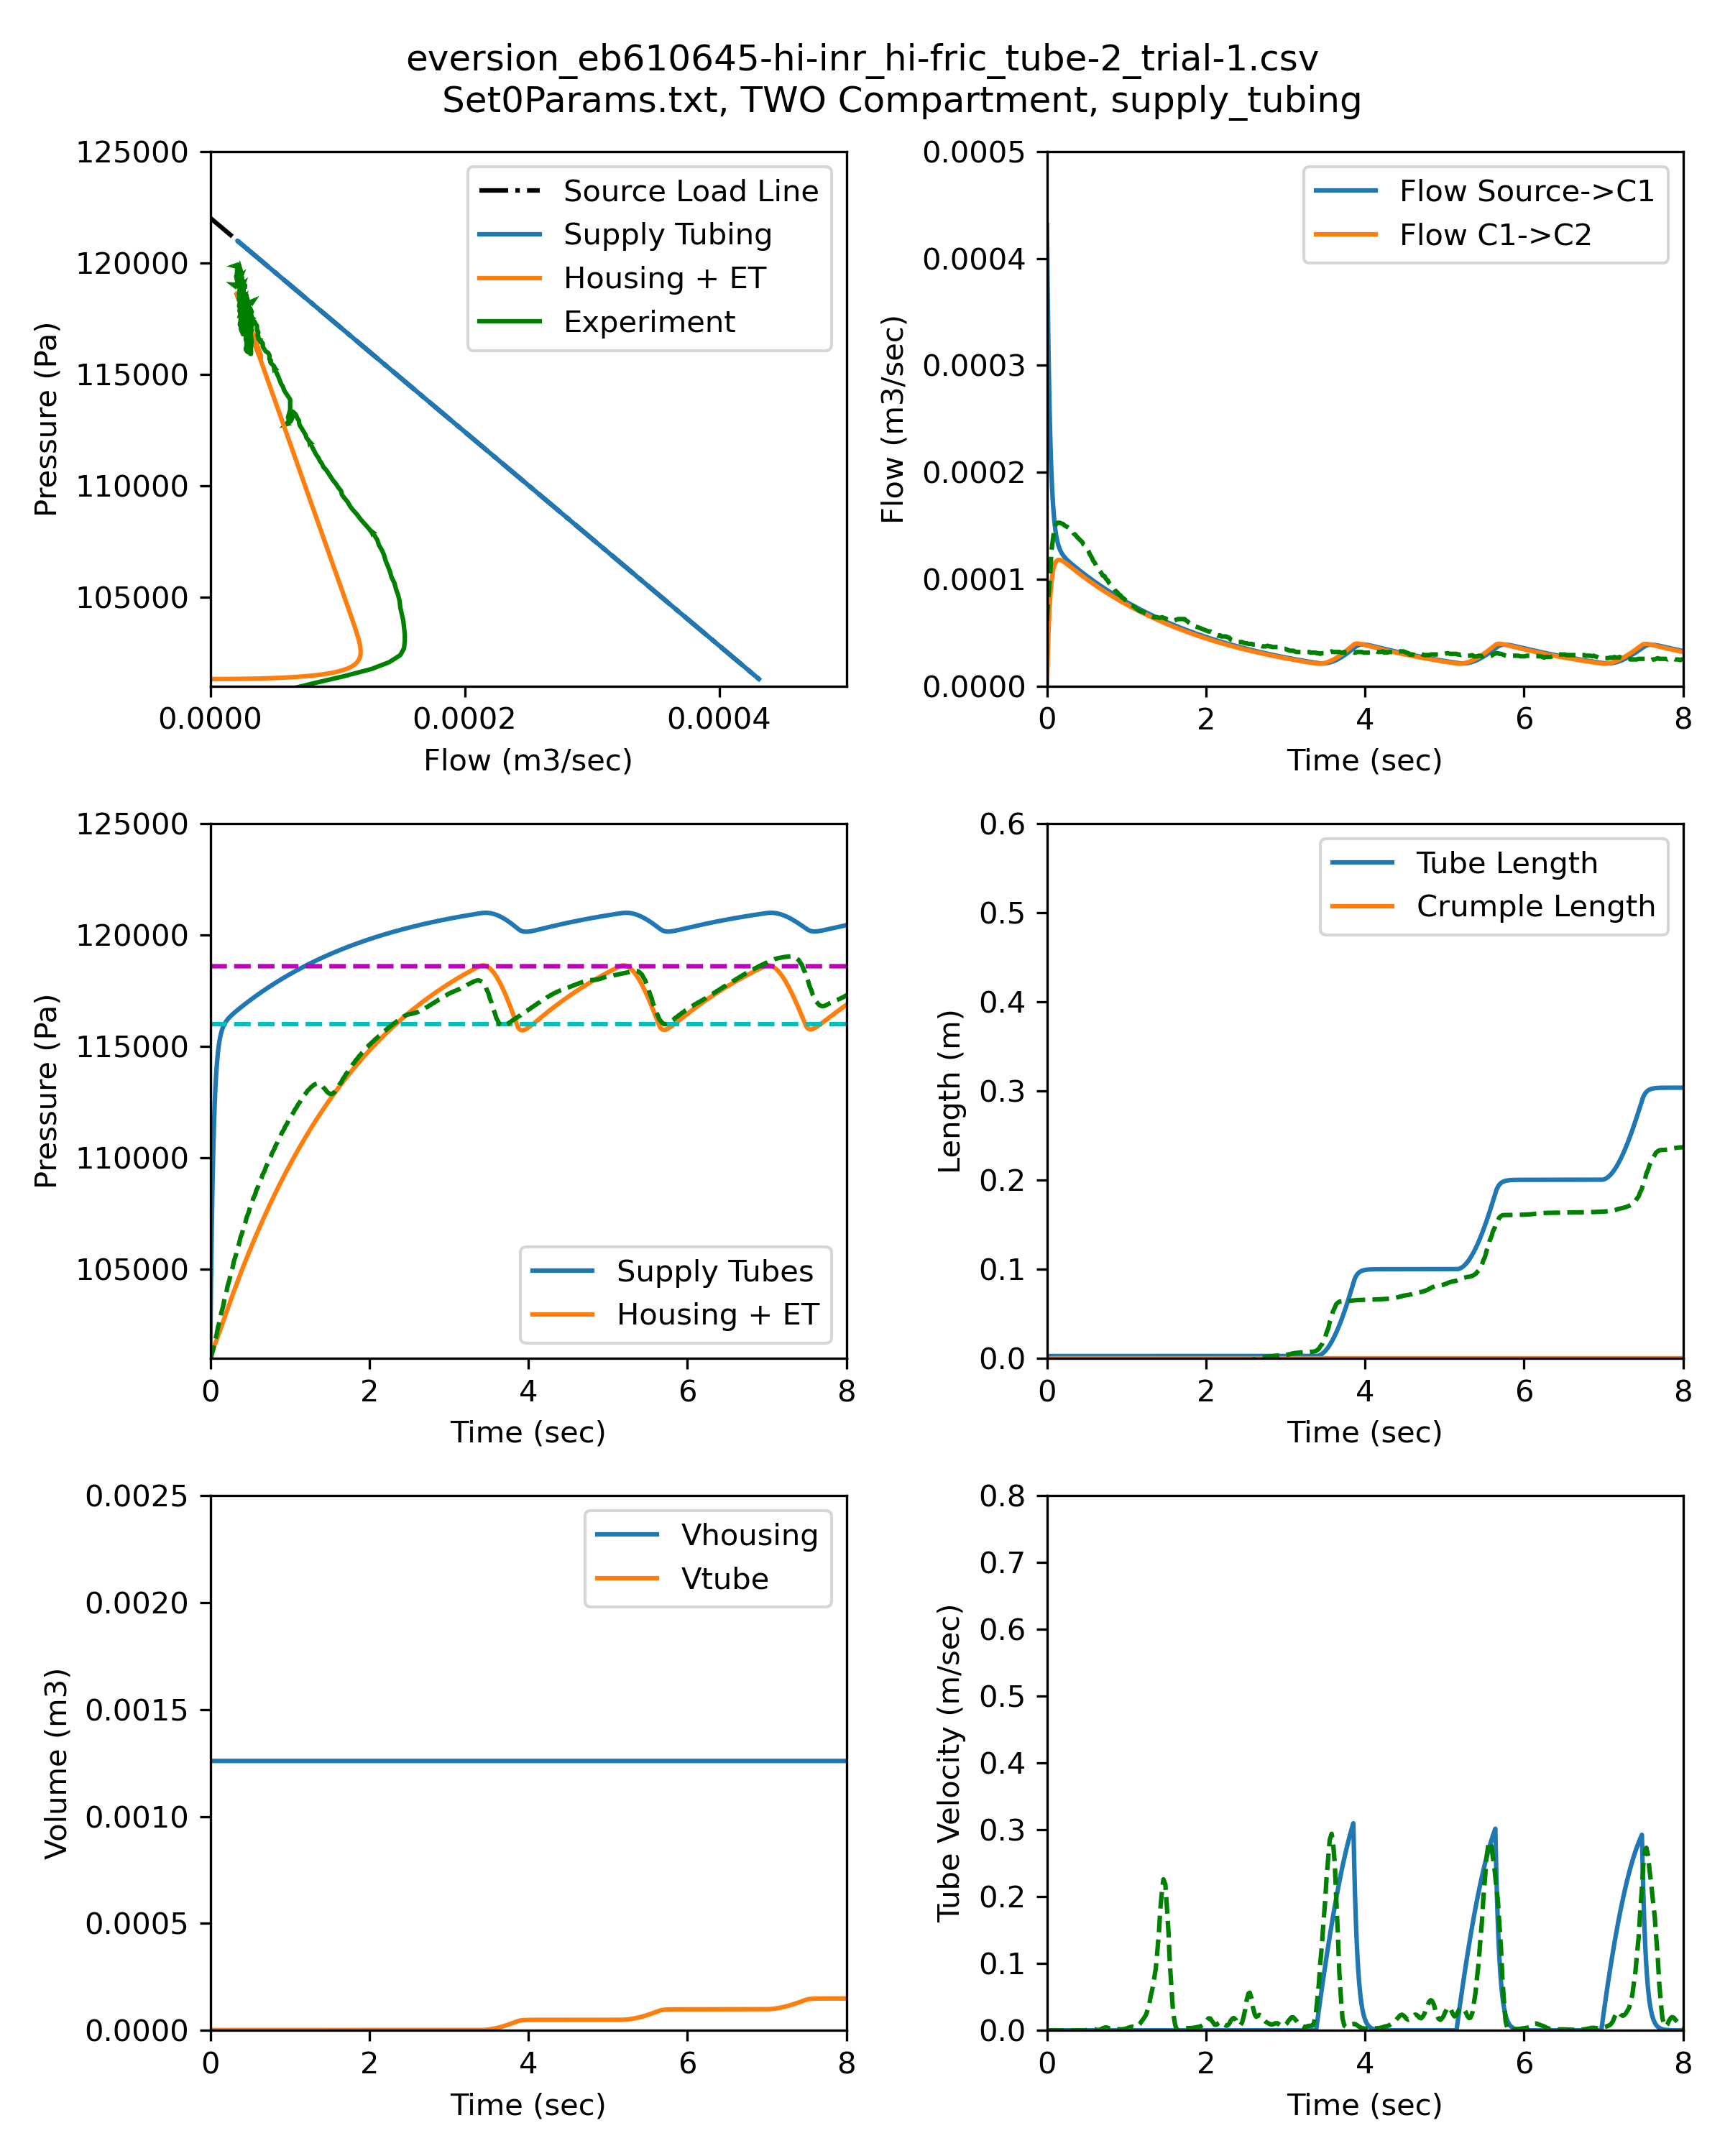
\includegraphics[width=0.475\textwidth]{9Files_Sim_outputs/Set0redo-26-Aug.png}
\includegraphics[width=0.475\textwidth]{9Files_Sim_outputs/Set1redo22-Aug.png}
\caption{Simulations 0 and 1.}
\end{figure}

\clearpage
\begin{figure}\centering
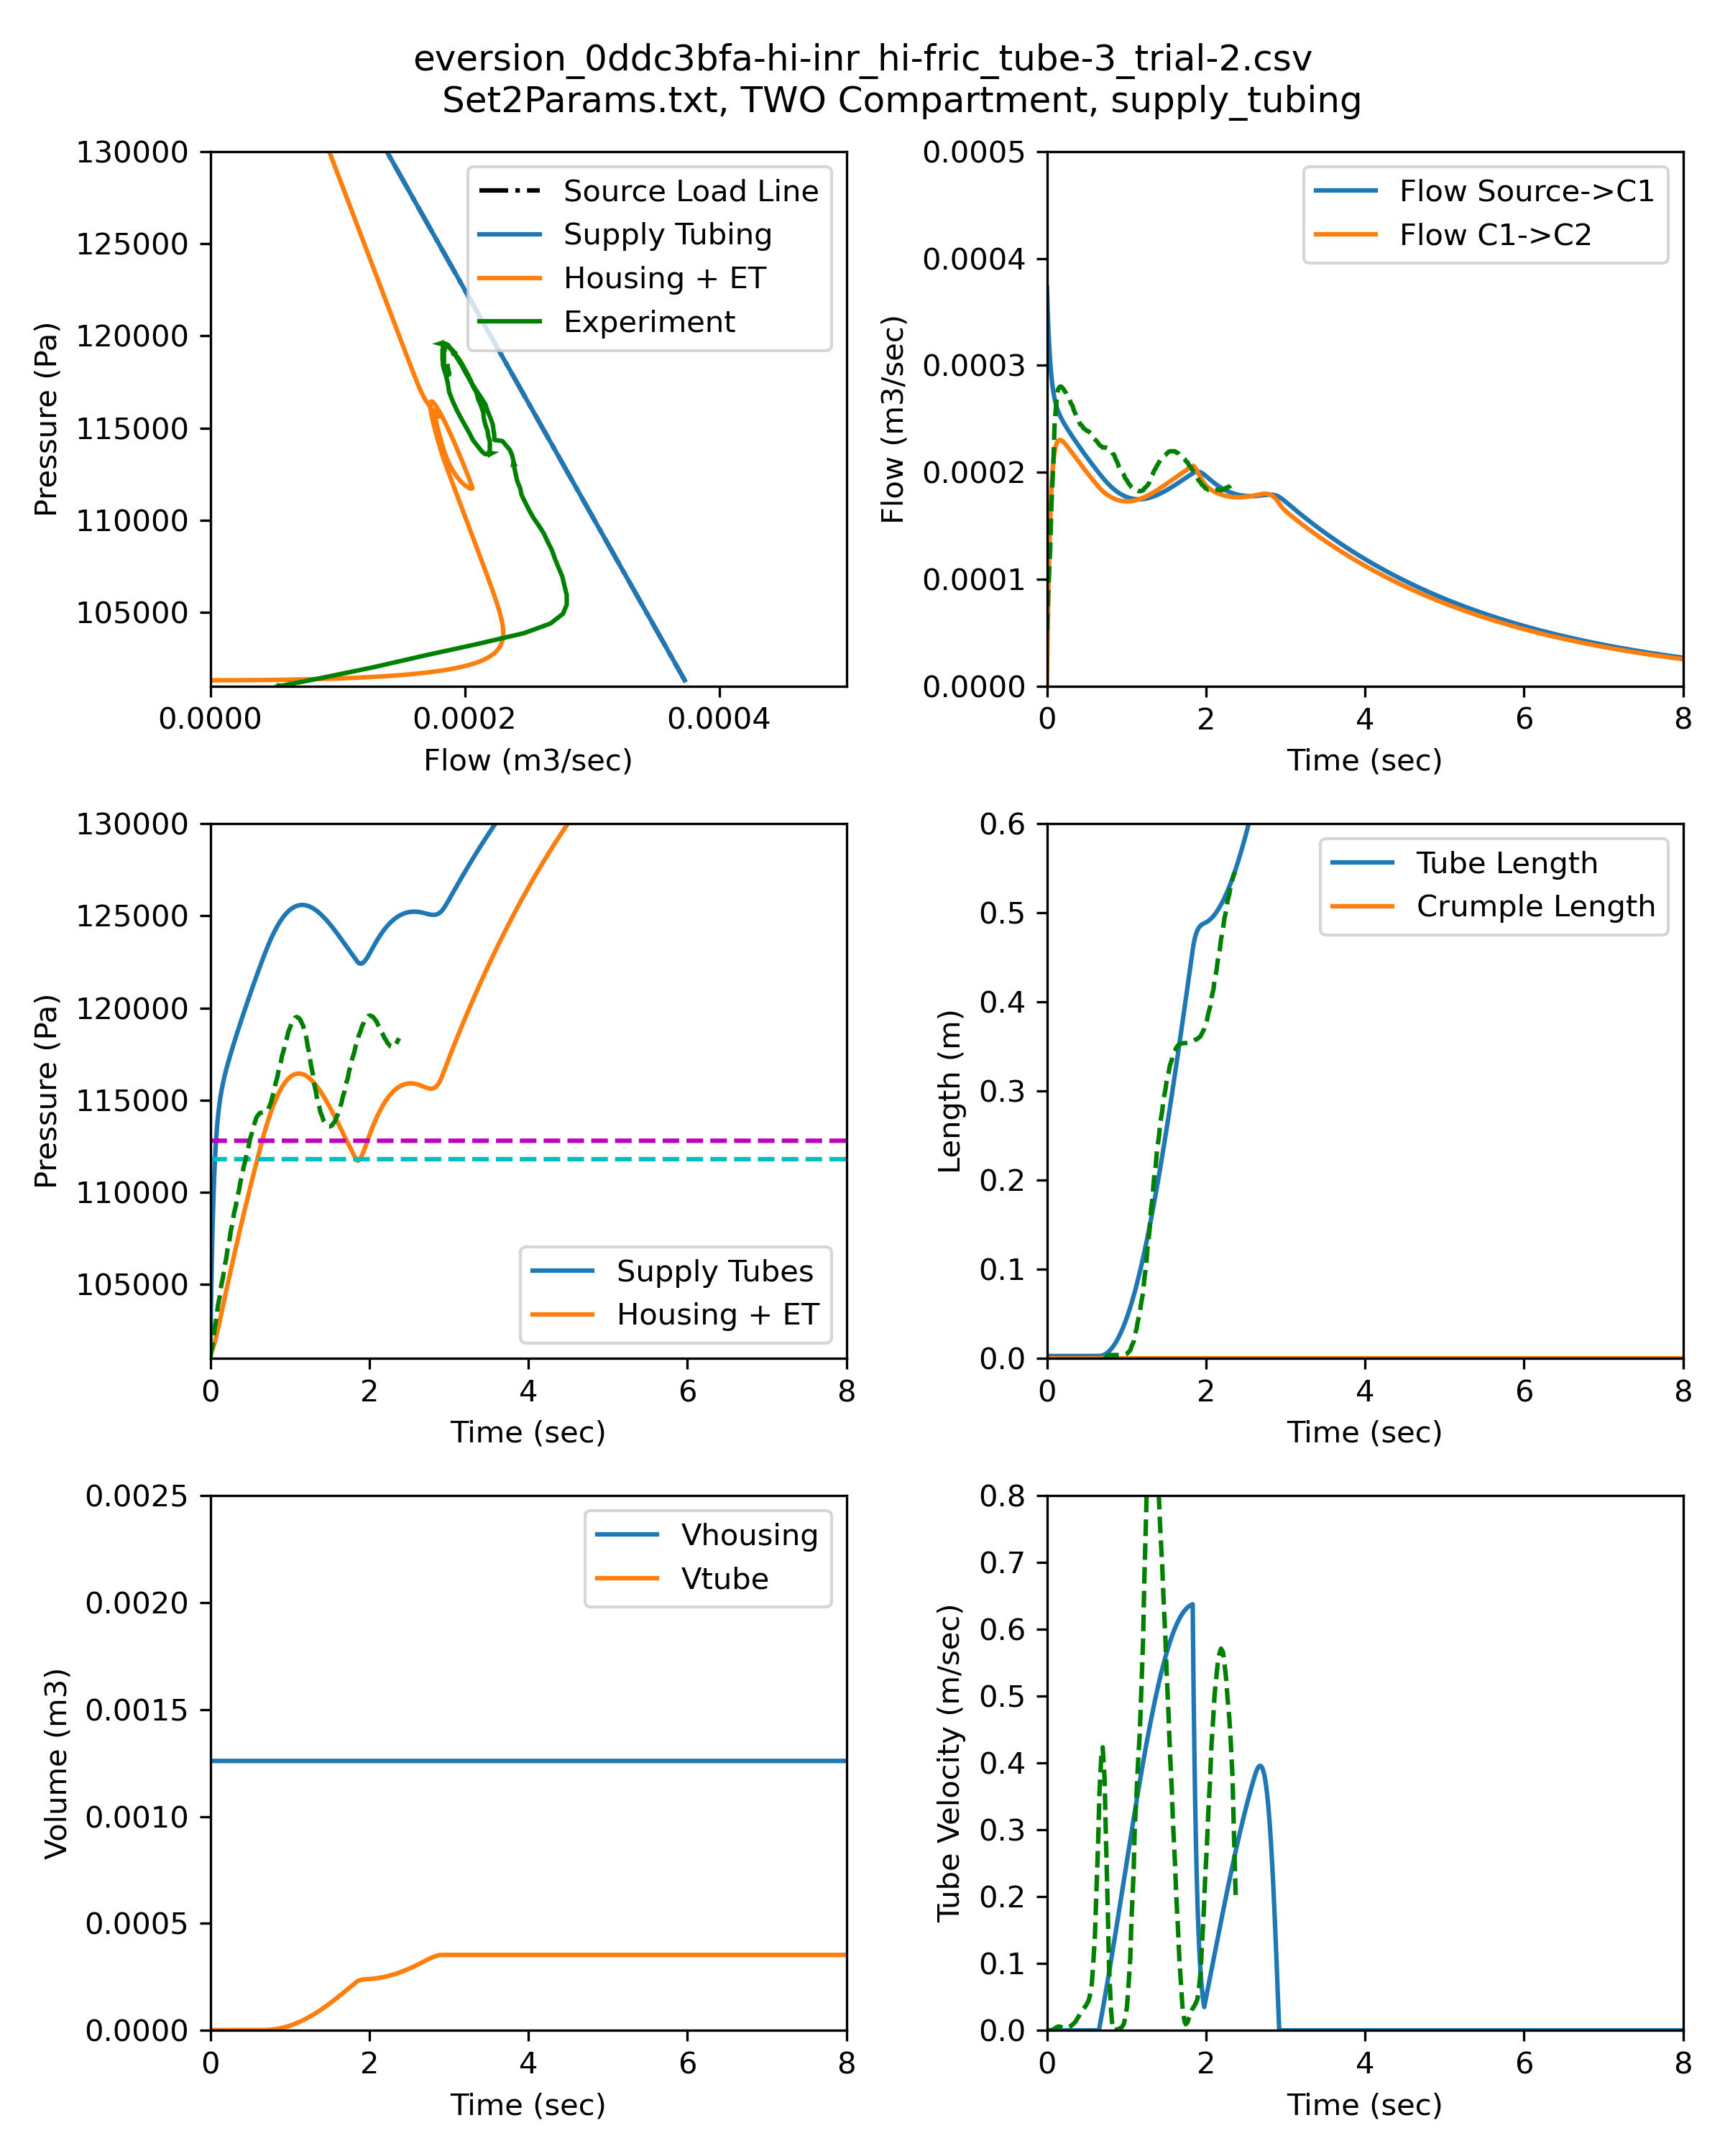
\includegraphics[width=0.475\textwidth]{9Files_Sim_outputs/Set2redo22-Aug.png}
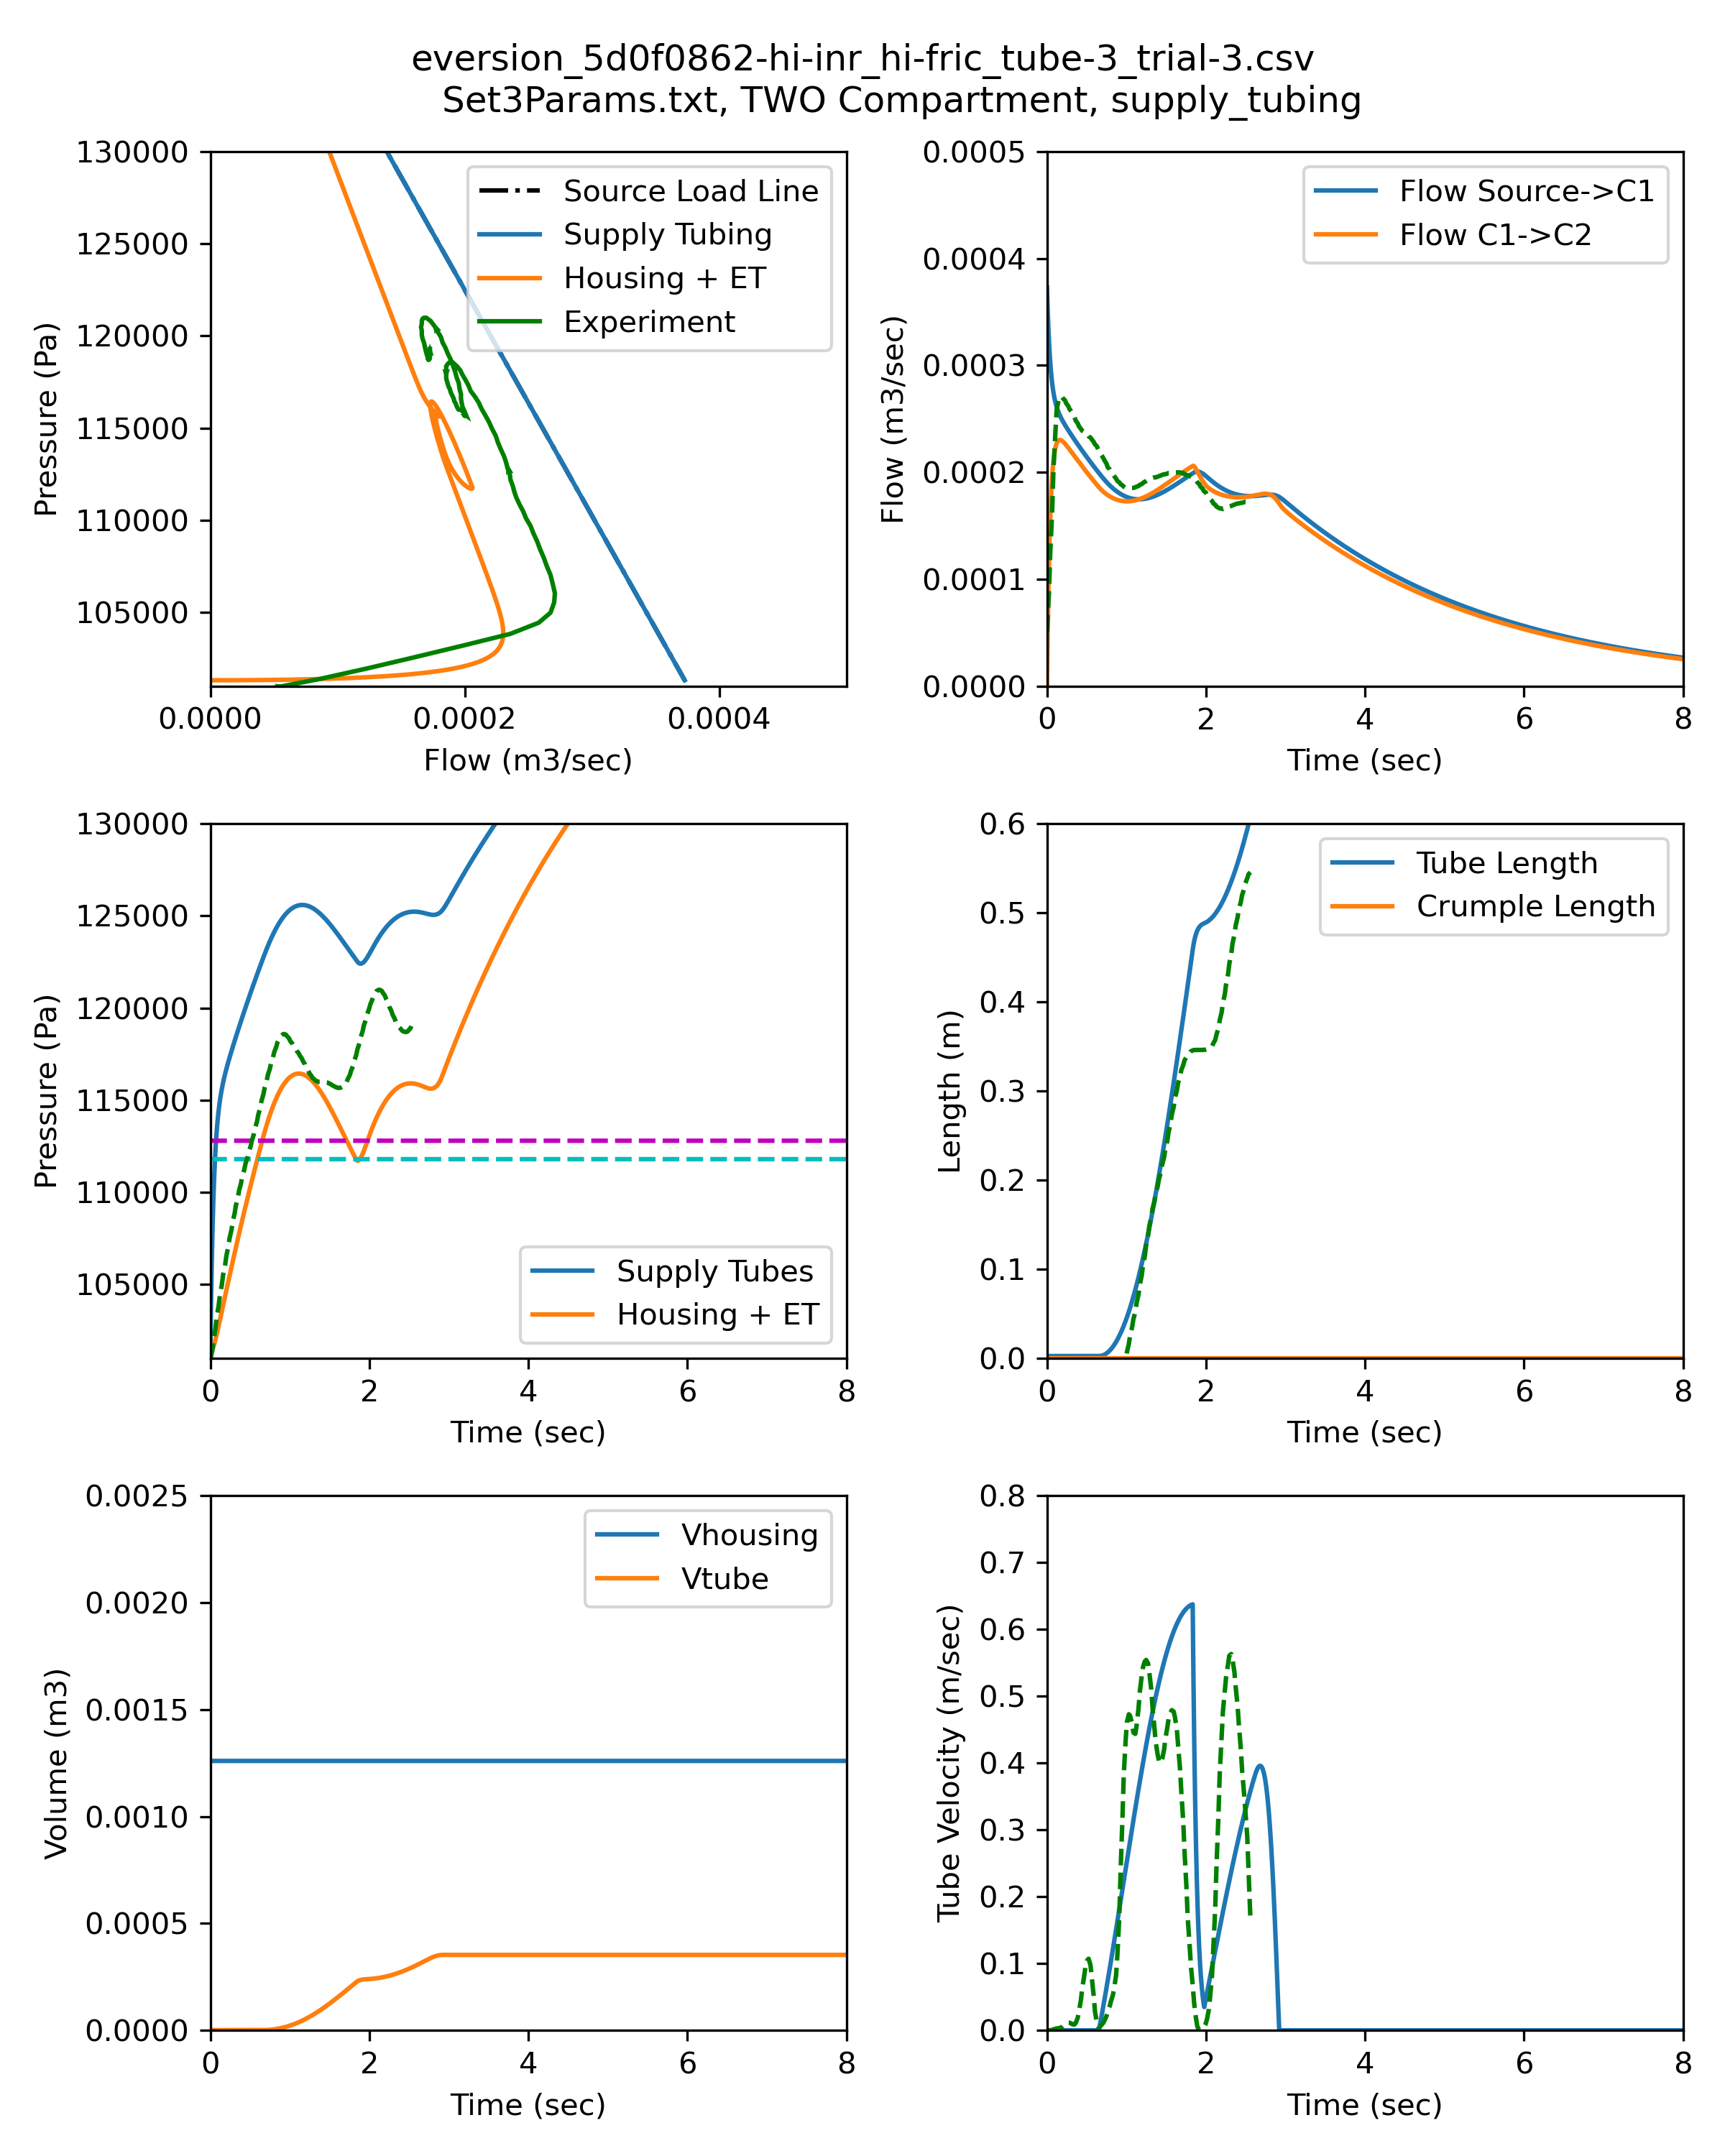
\includegraphics[width=0.475\textwidth]{9Files_Sim_outputs/Set3redo22-Aug.png}
\caption{Simulations 2 and 3.}
\end{figure}


\begin{figure}\centering
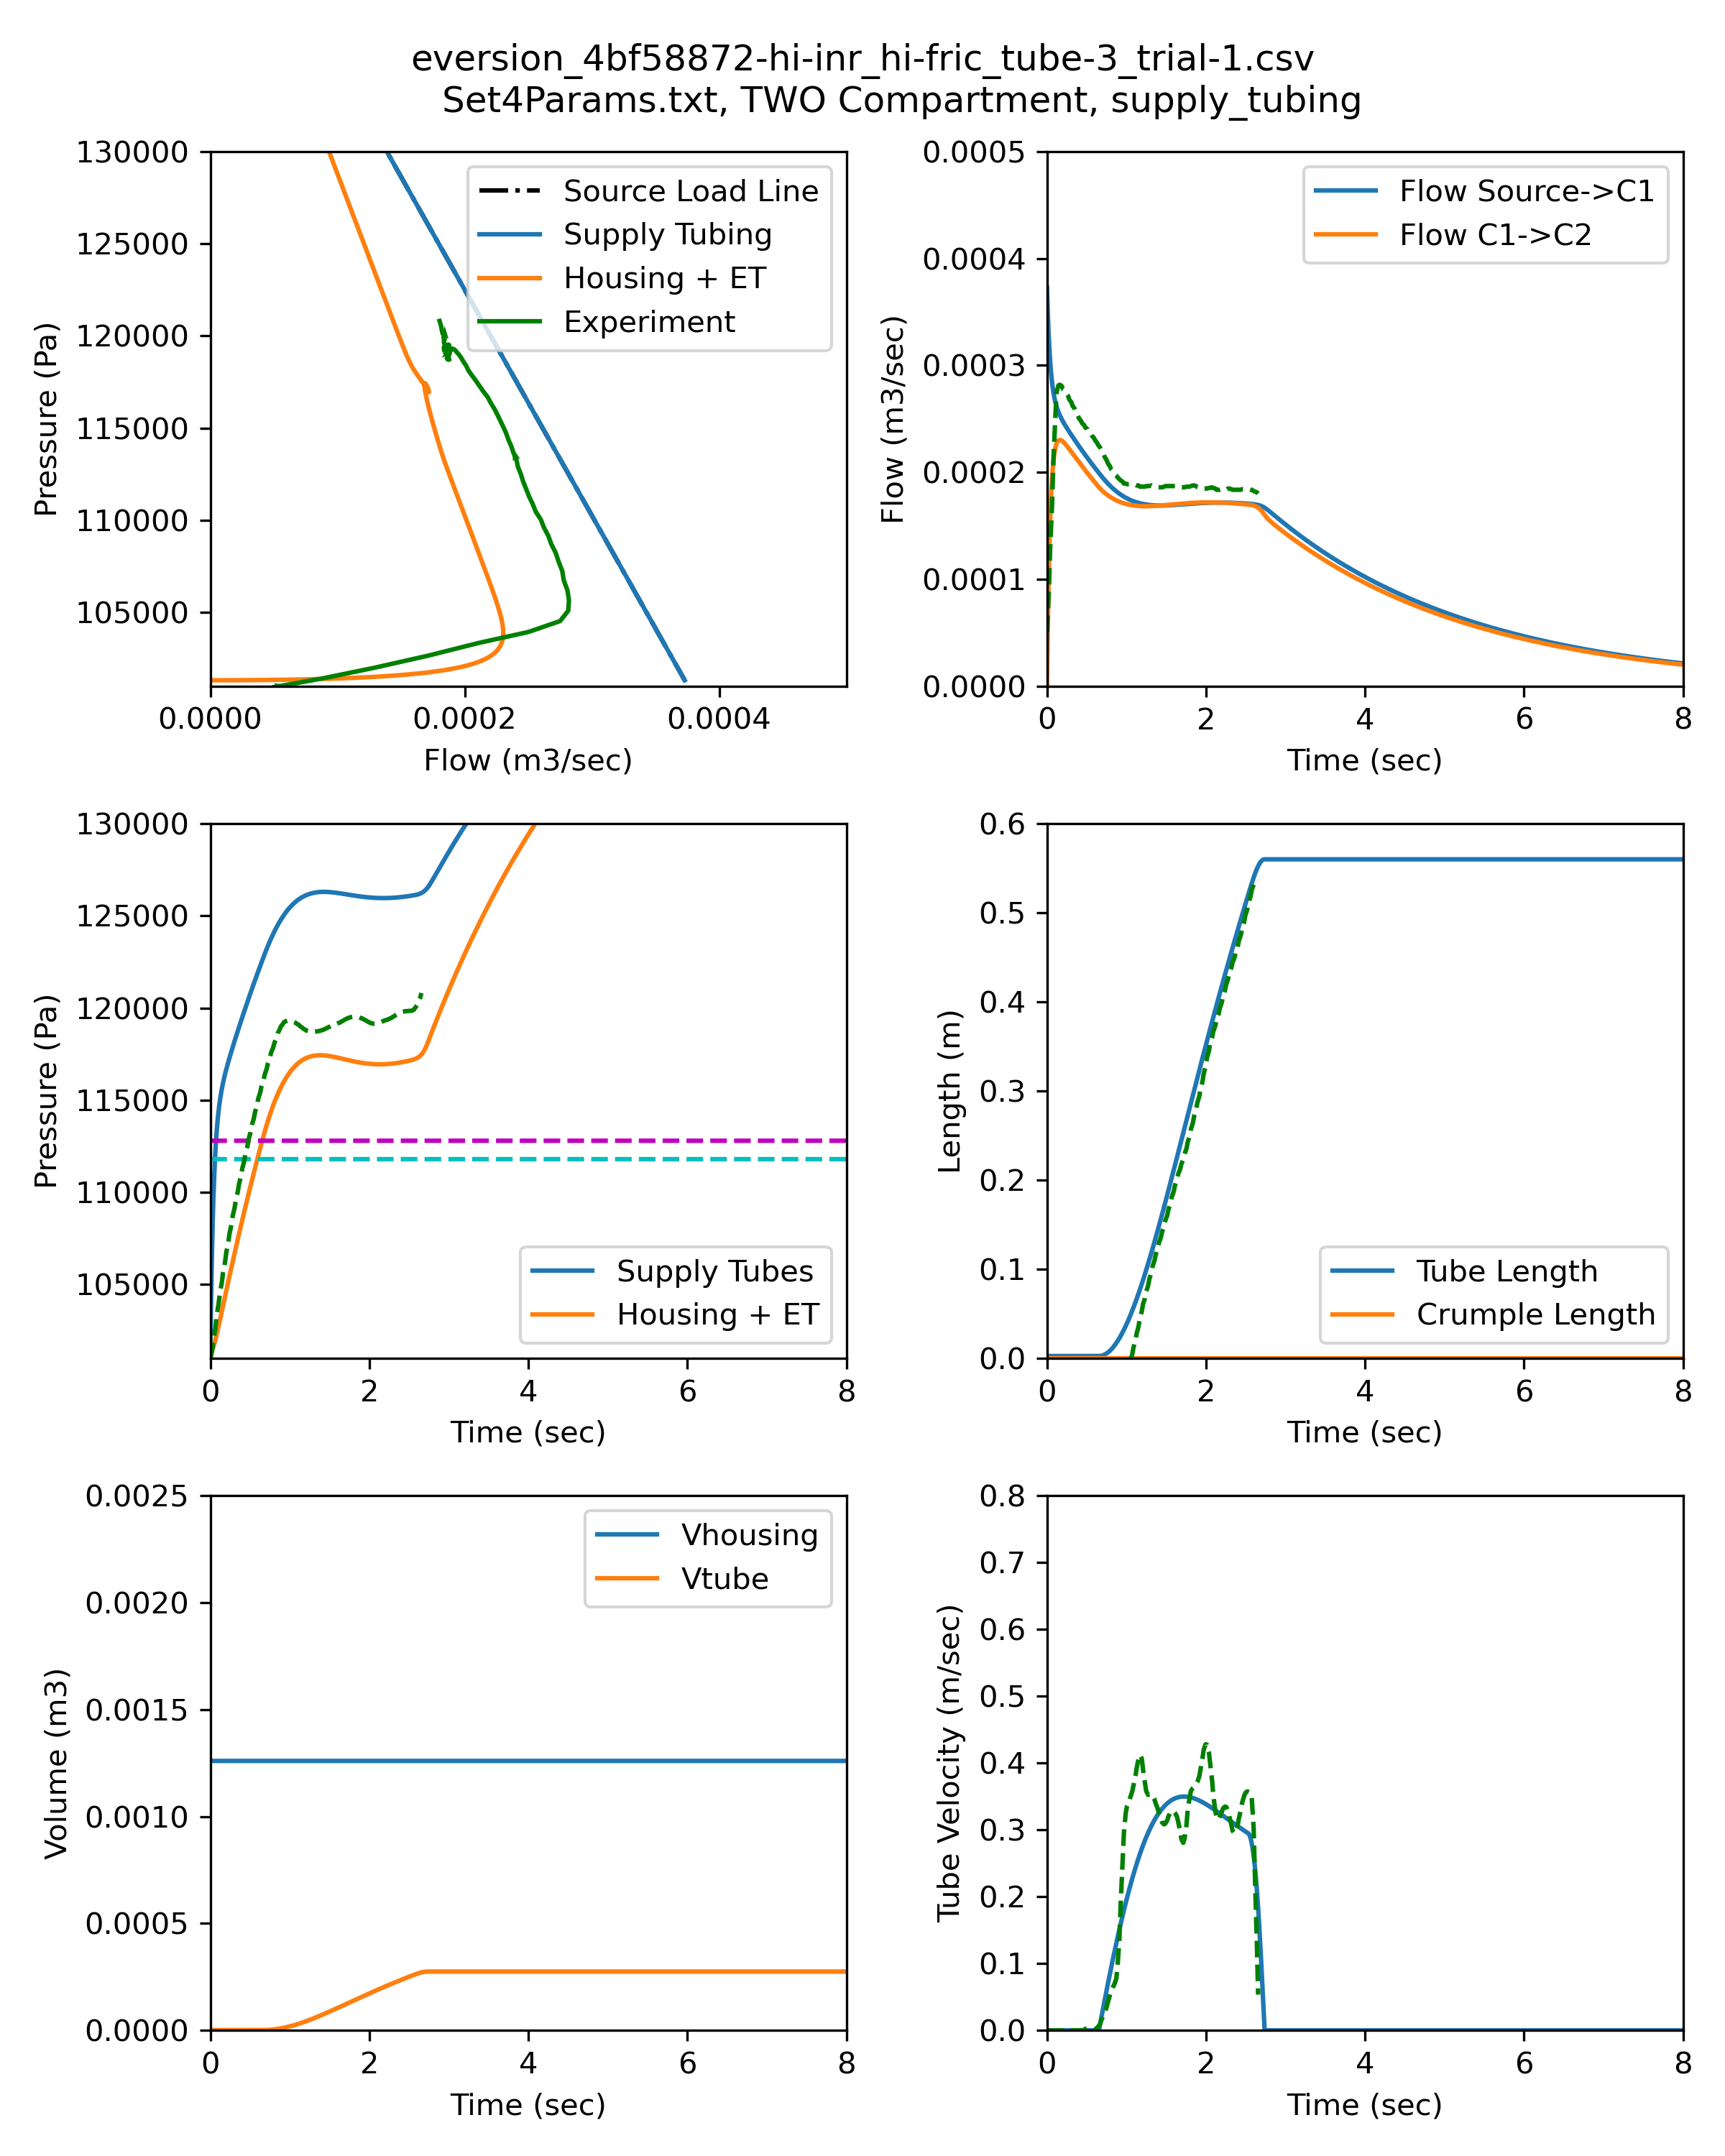
\includegraphics[width=0.475\textwidth]{9Files_Sim_outputs/Set4redo22-Aug.png}
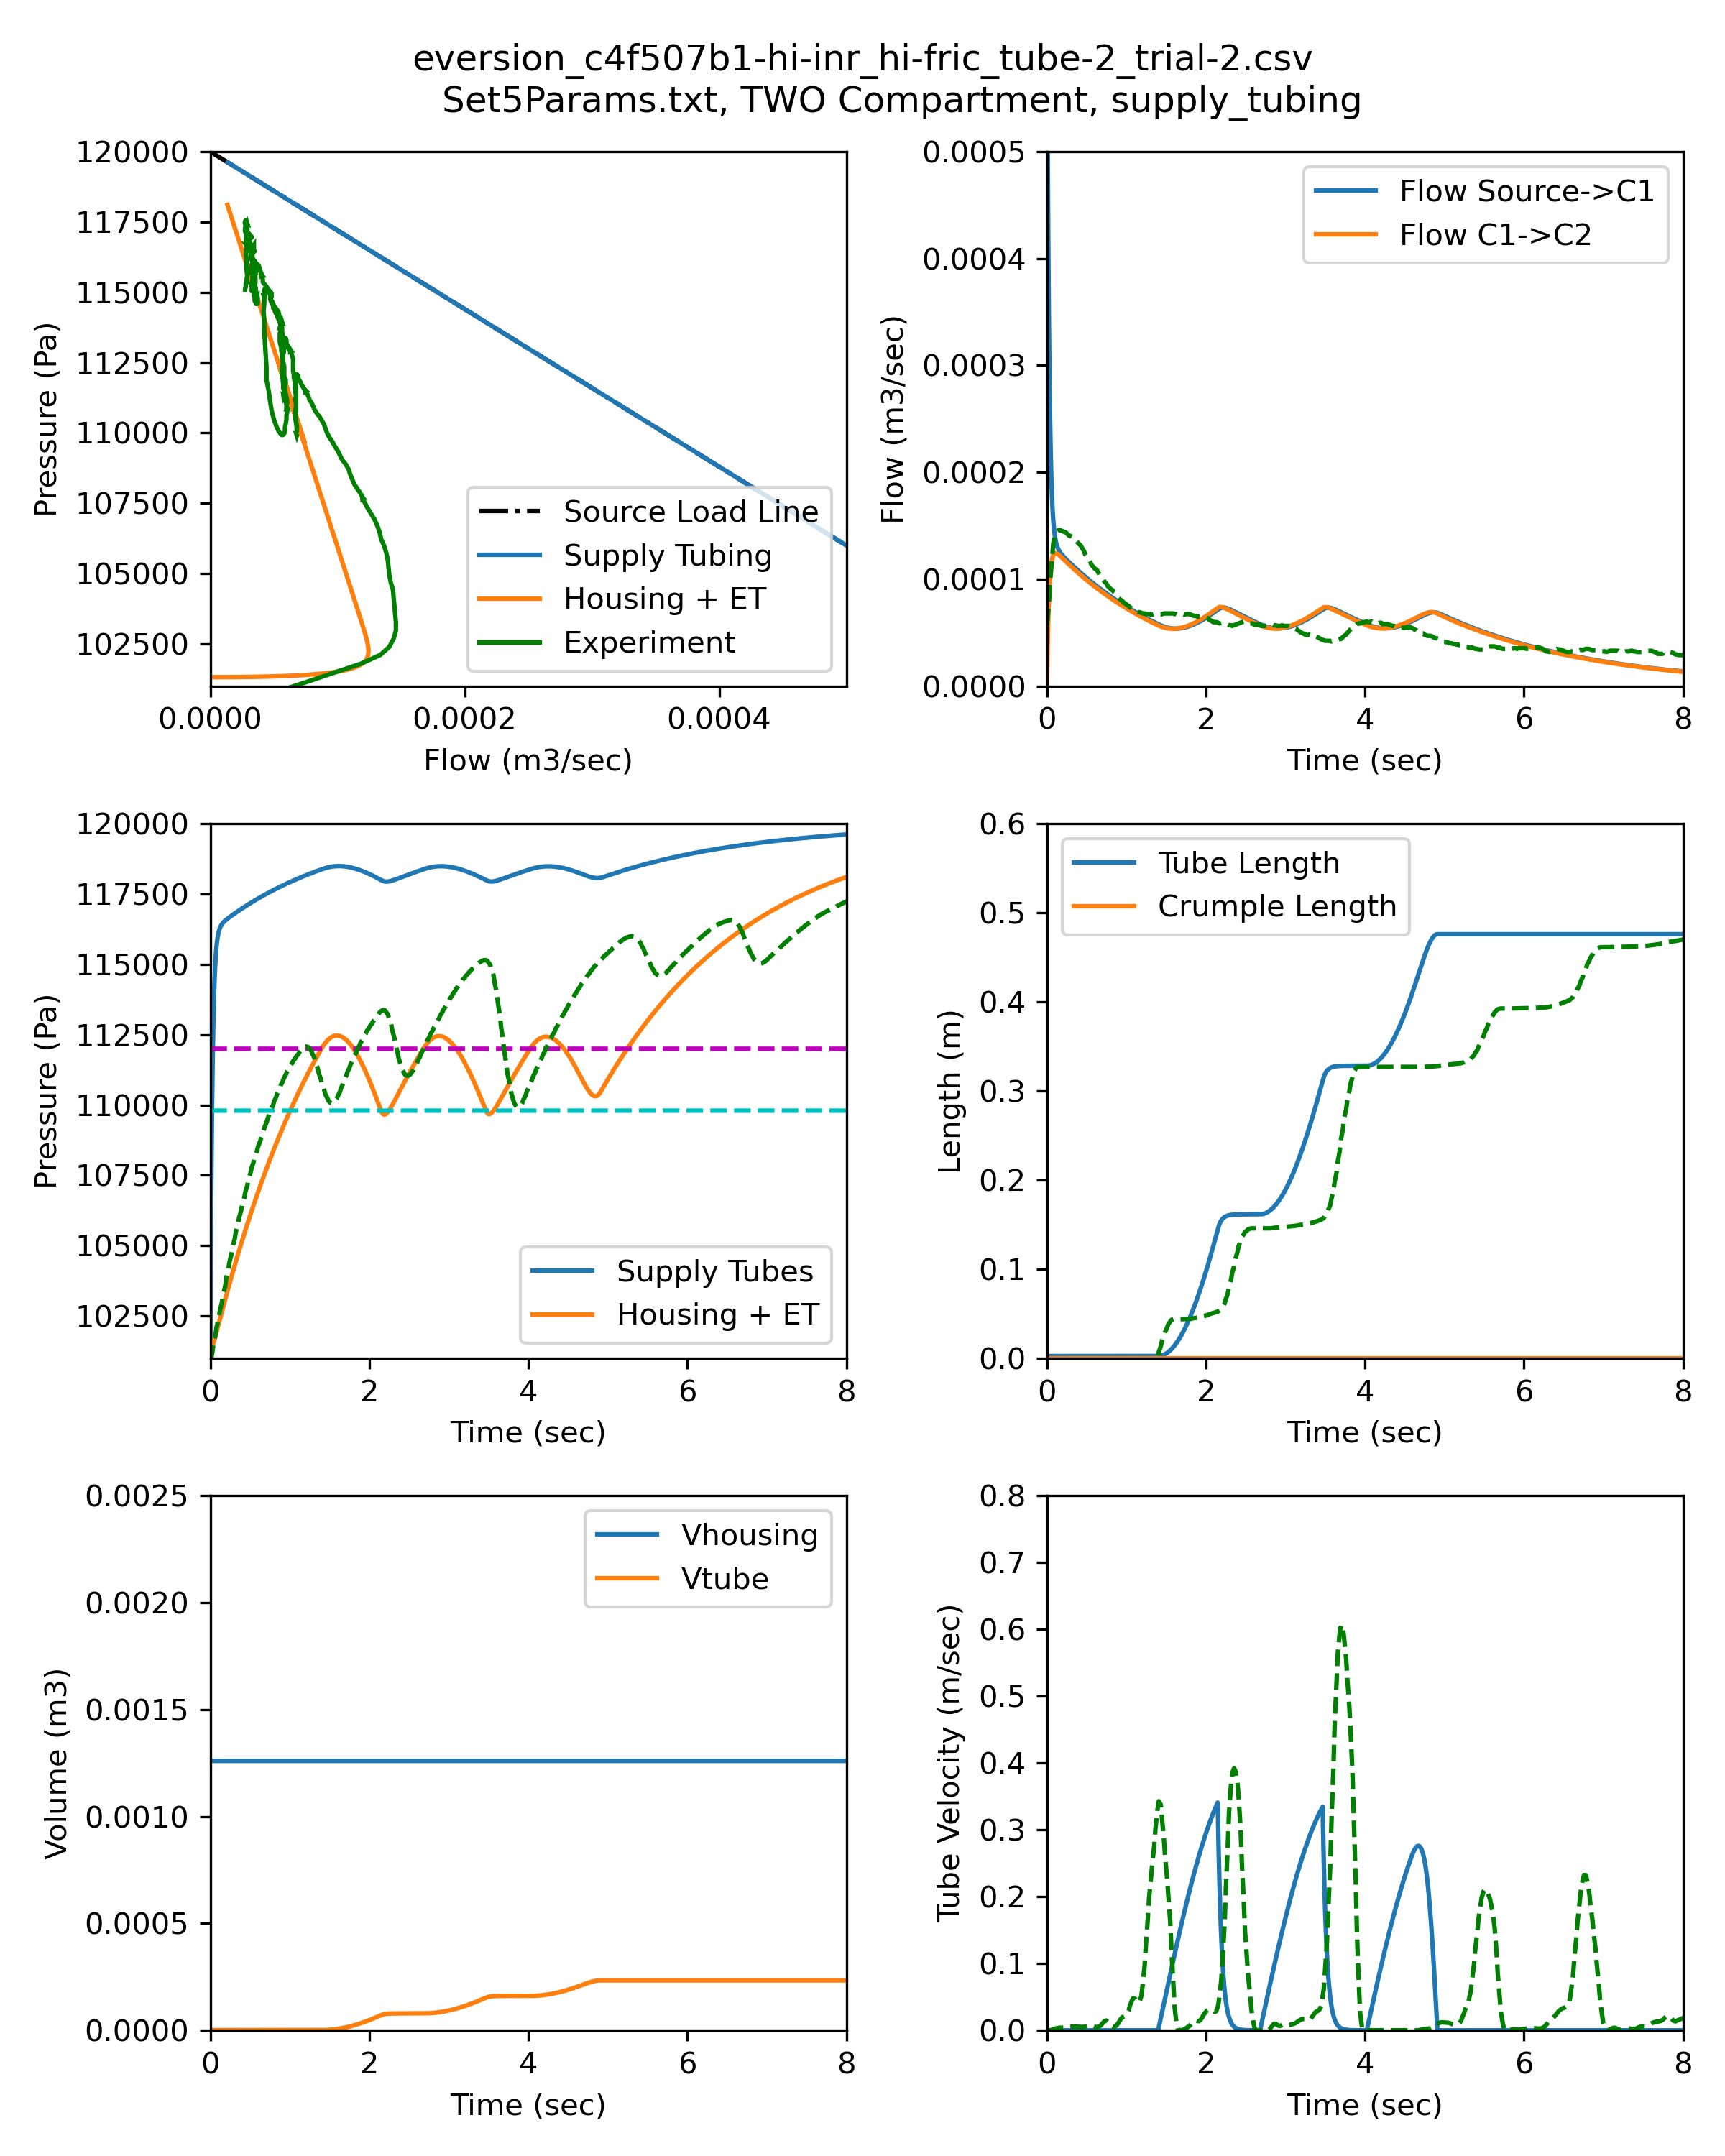
\includegraphics[width=0.475\textwidth]{9Files_Sim_outputs/Set5redo22-Aug.png}
\caption{Simulations 4 and 5.}
\end{figure}


\begin{figure}\centering
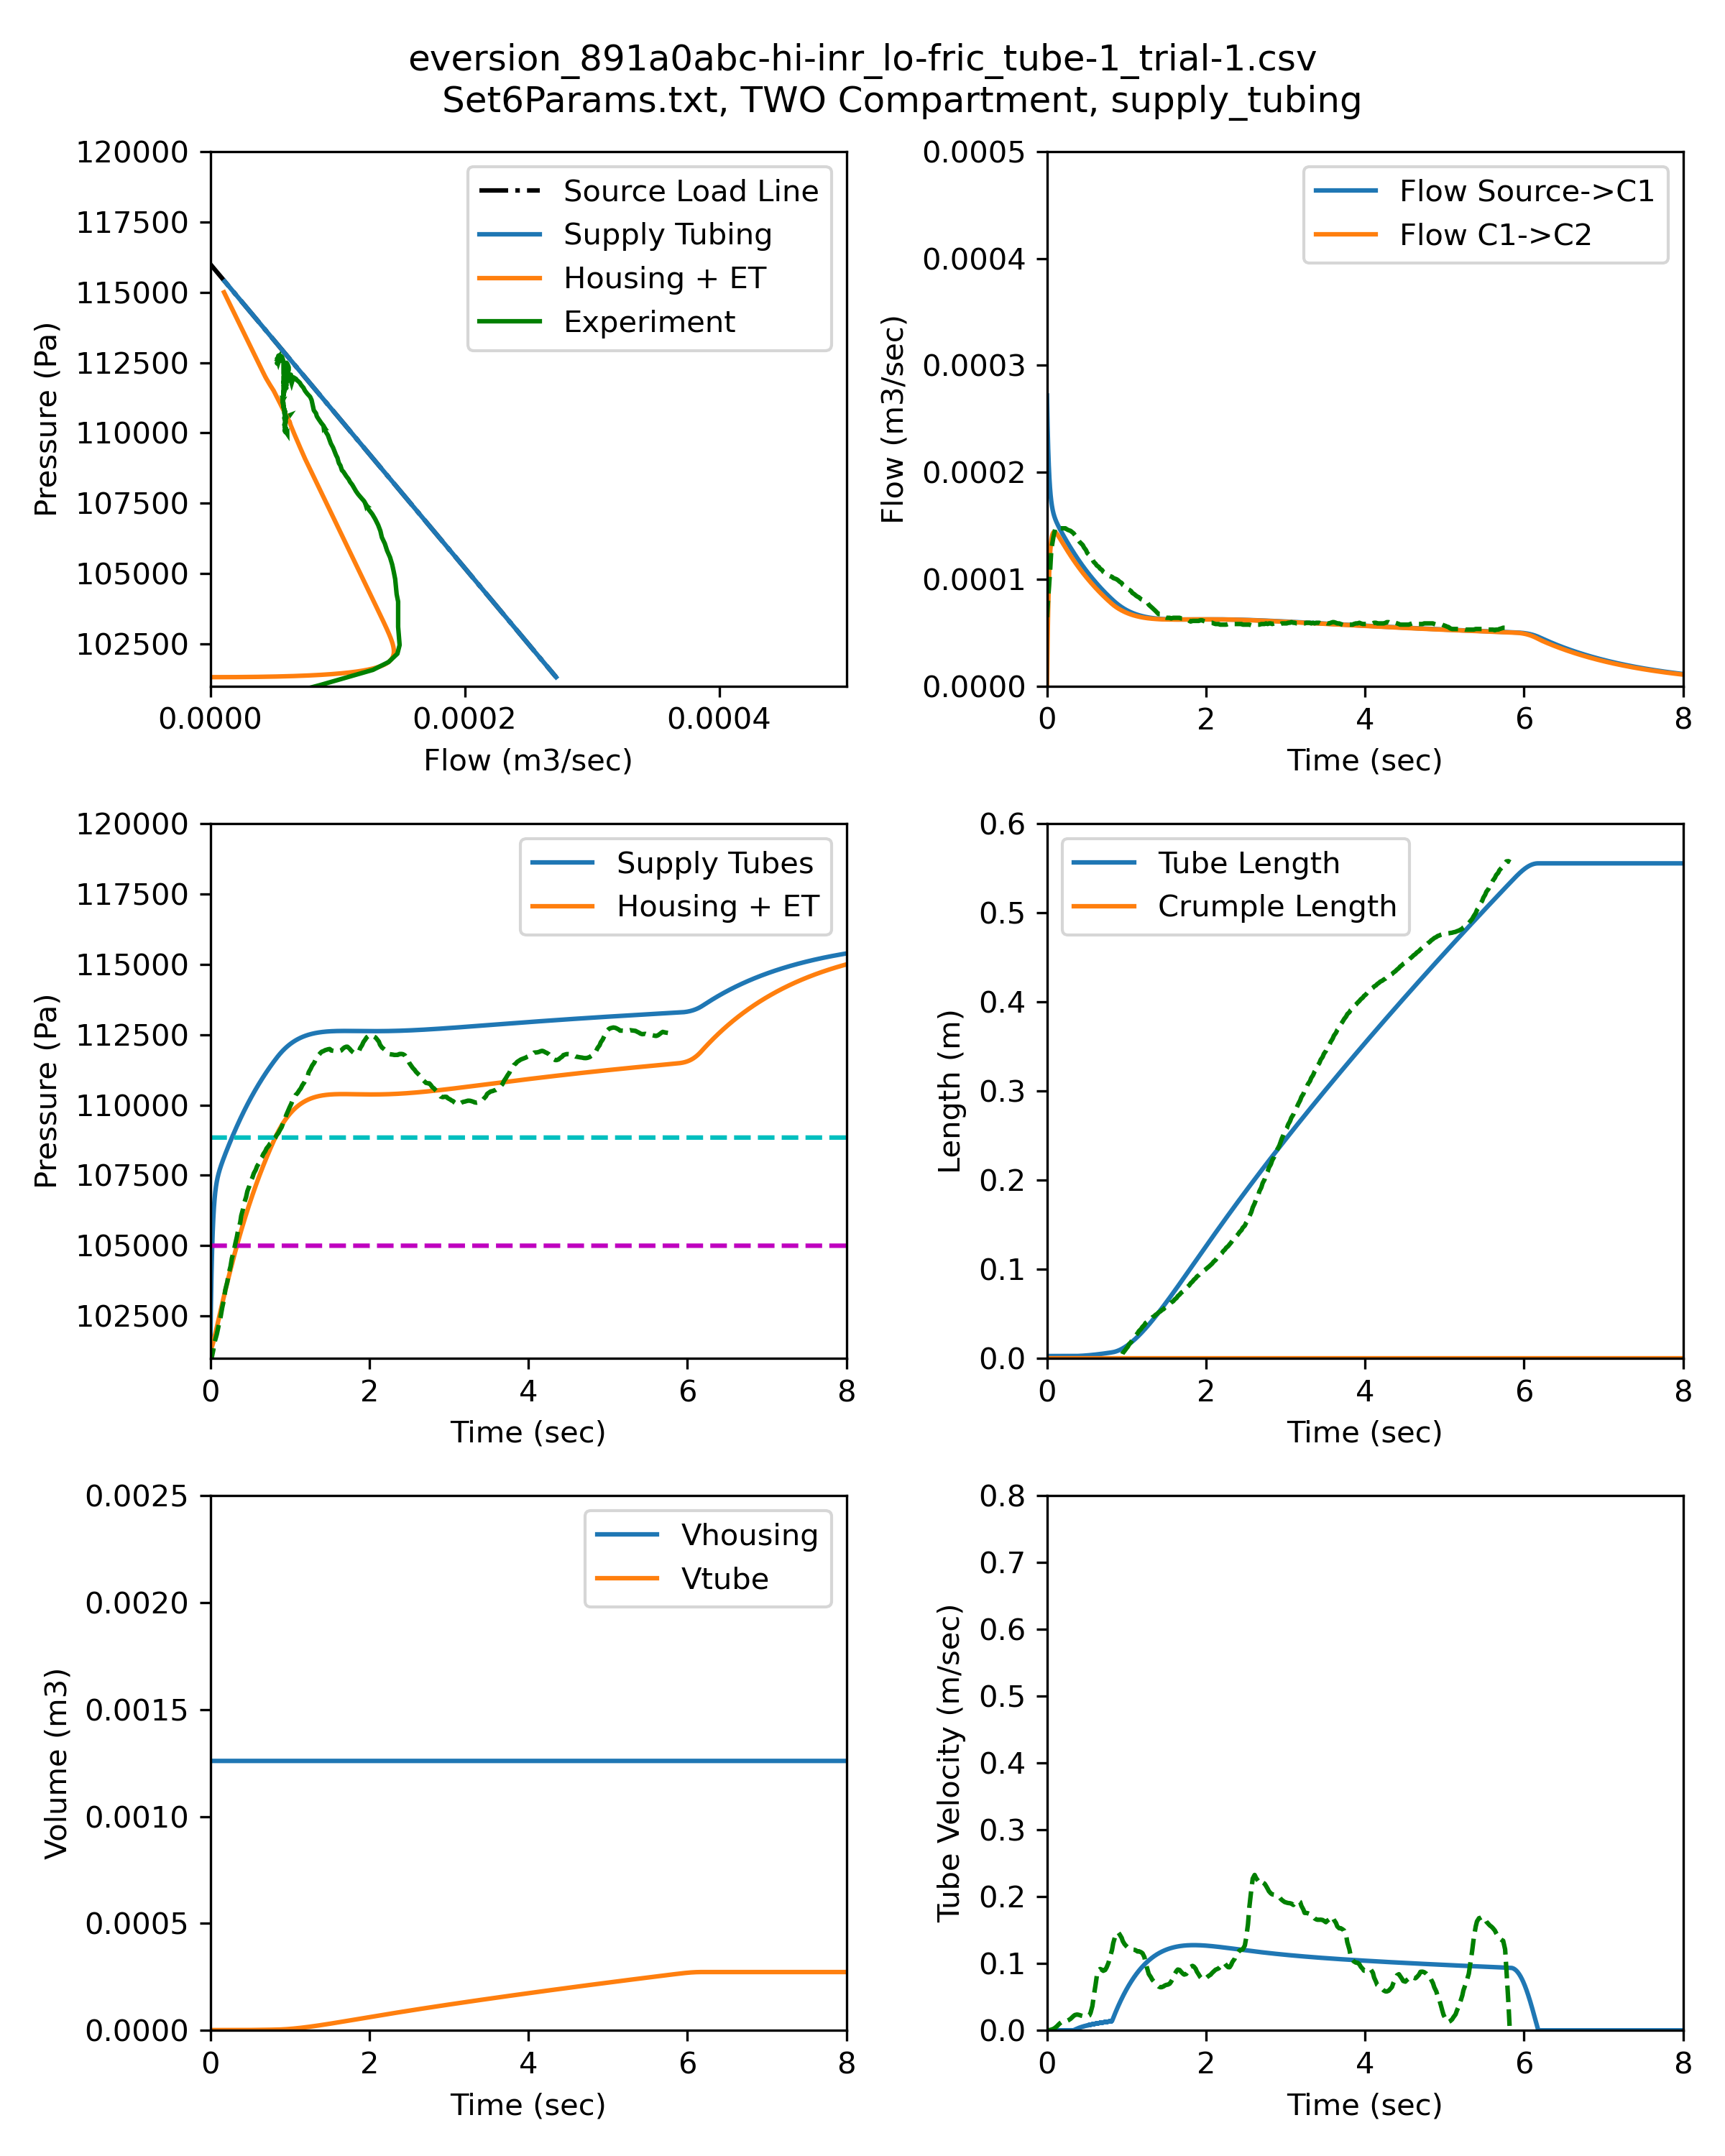
\includegraphics[width=0.475\textwidth]{9Files_Sim_outputs/Set6redo-26-Aug.png}
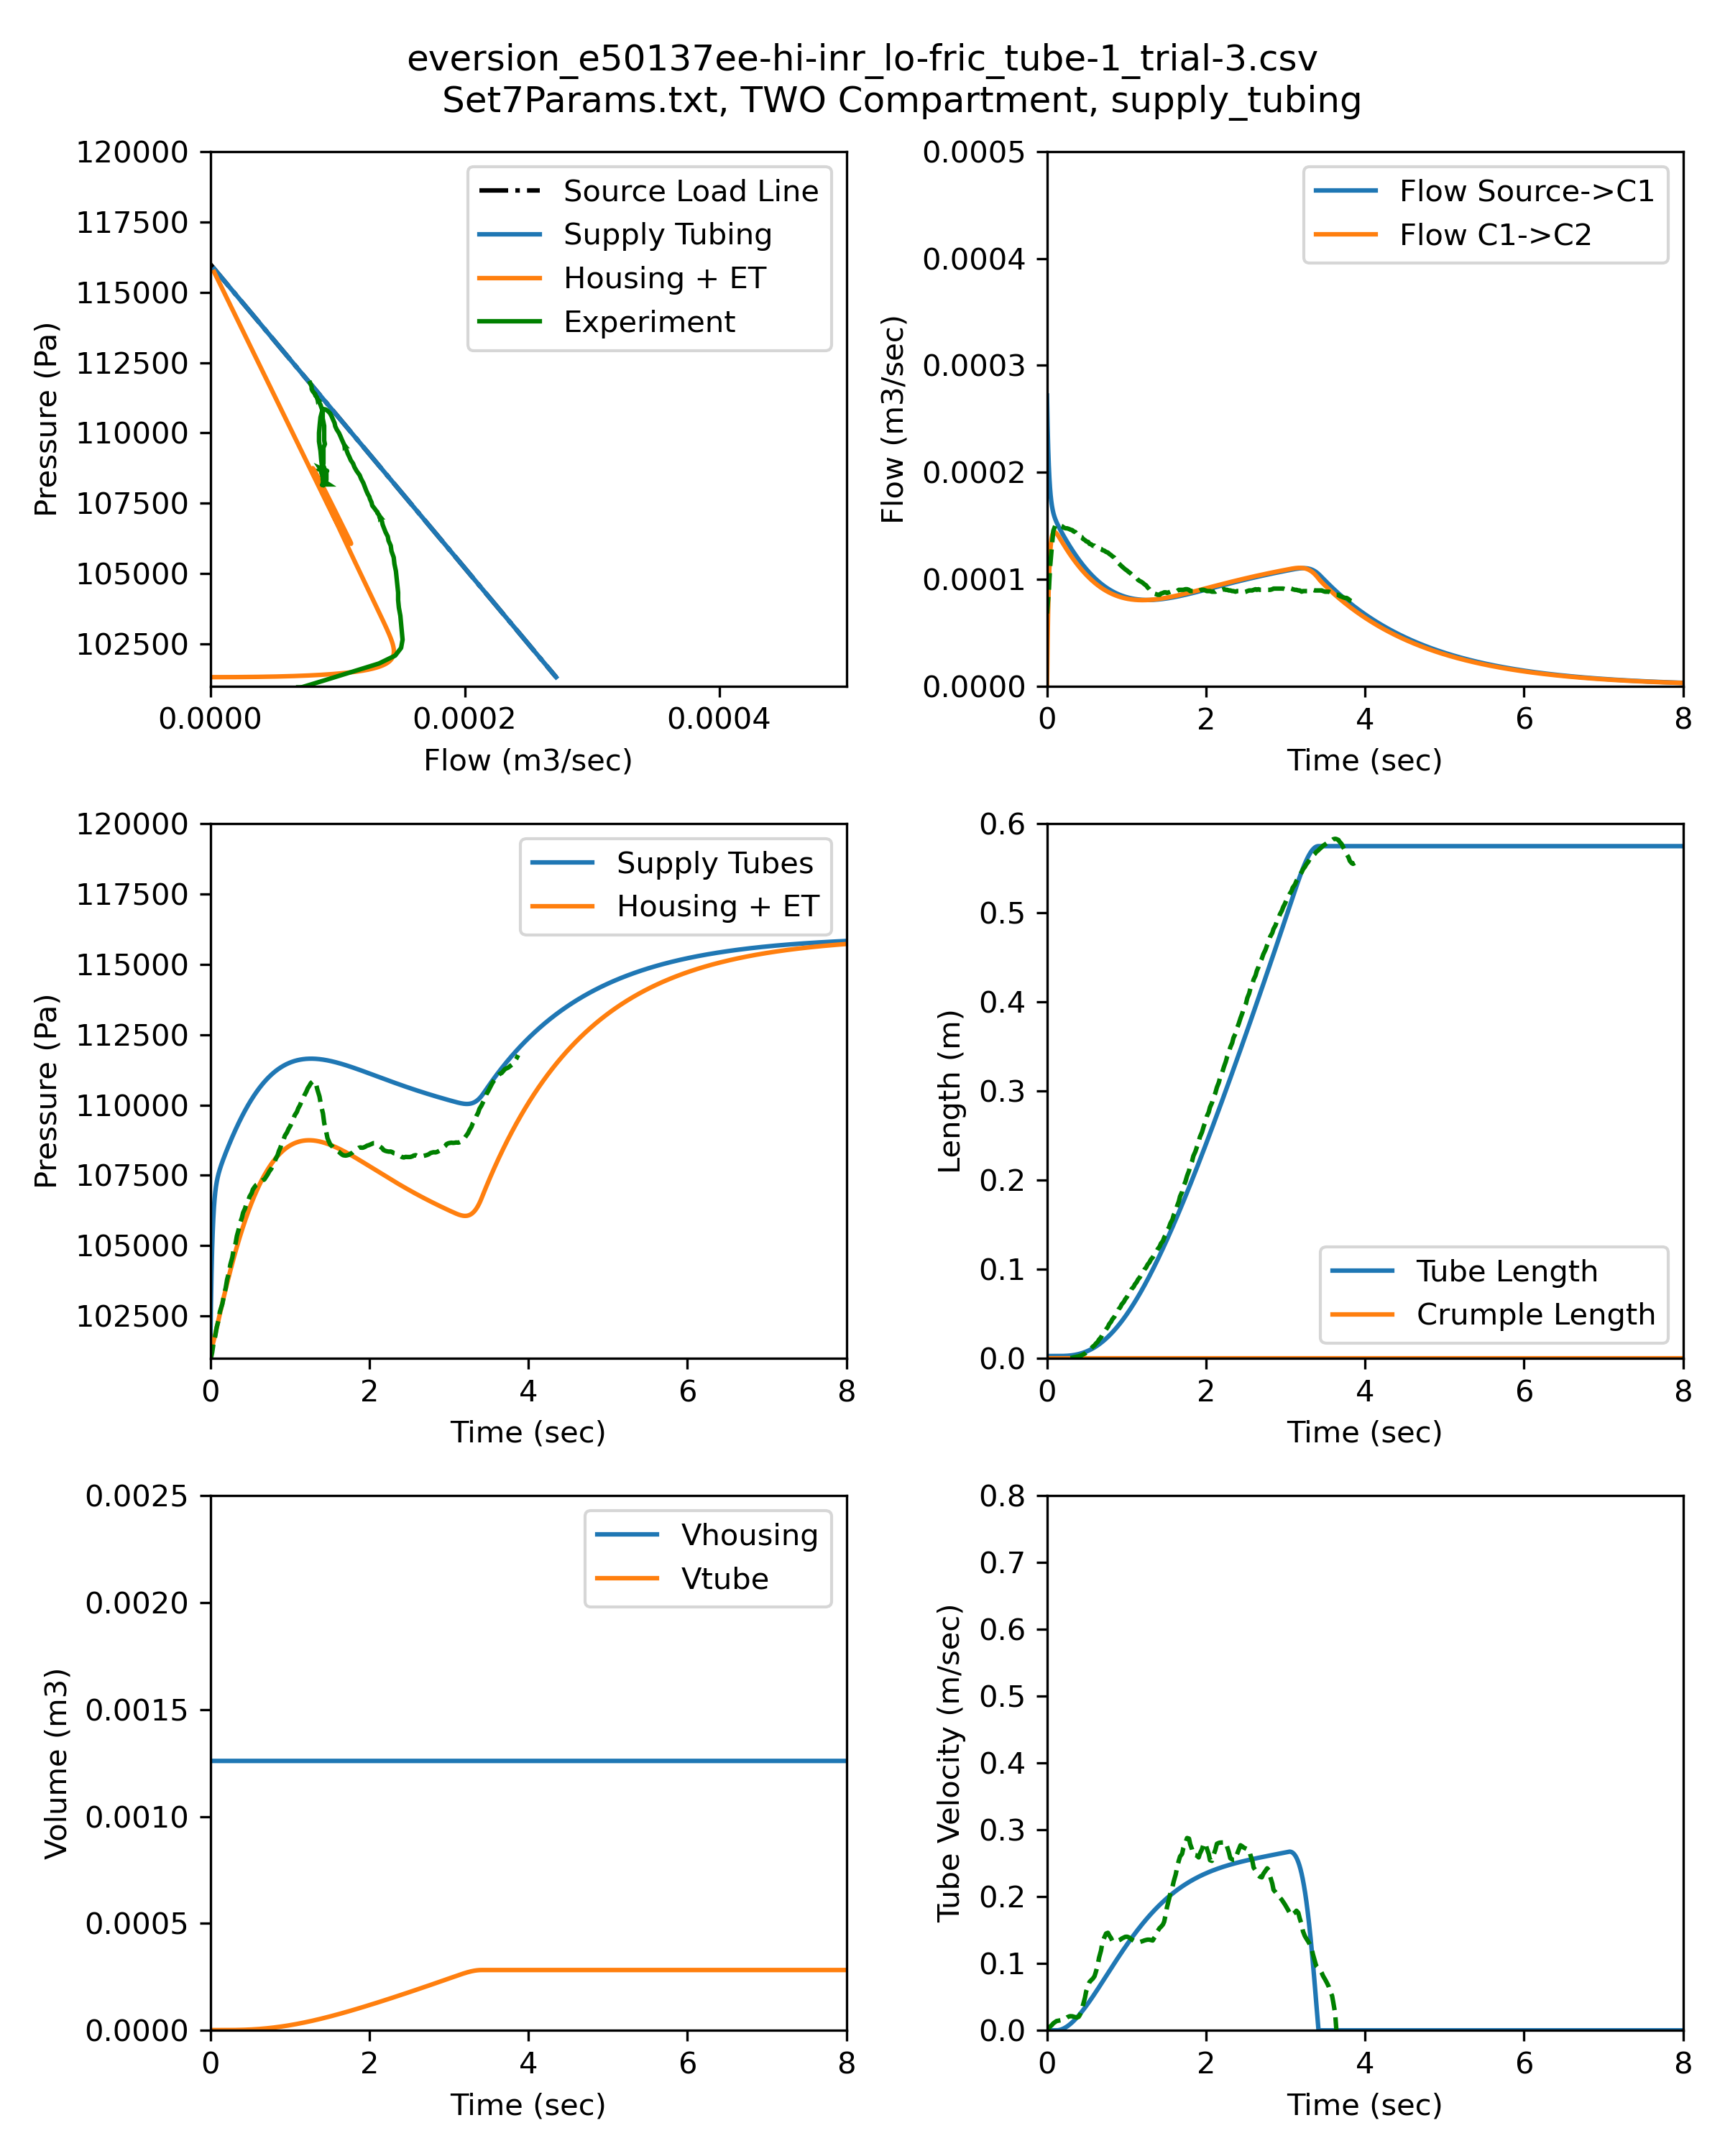
\includegraphics[width=0.475\textwidth]{9Files_Sim_outputs/Set7redo-26-Aug.png}
\caption{Simulations 6 and 7.}
\end{figure}



\begin{figure}\centering
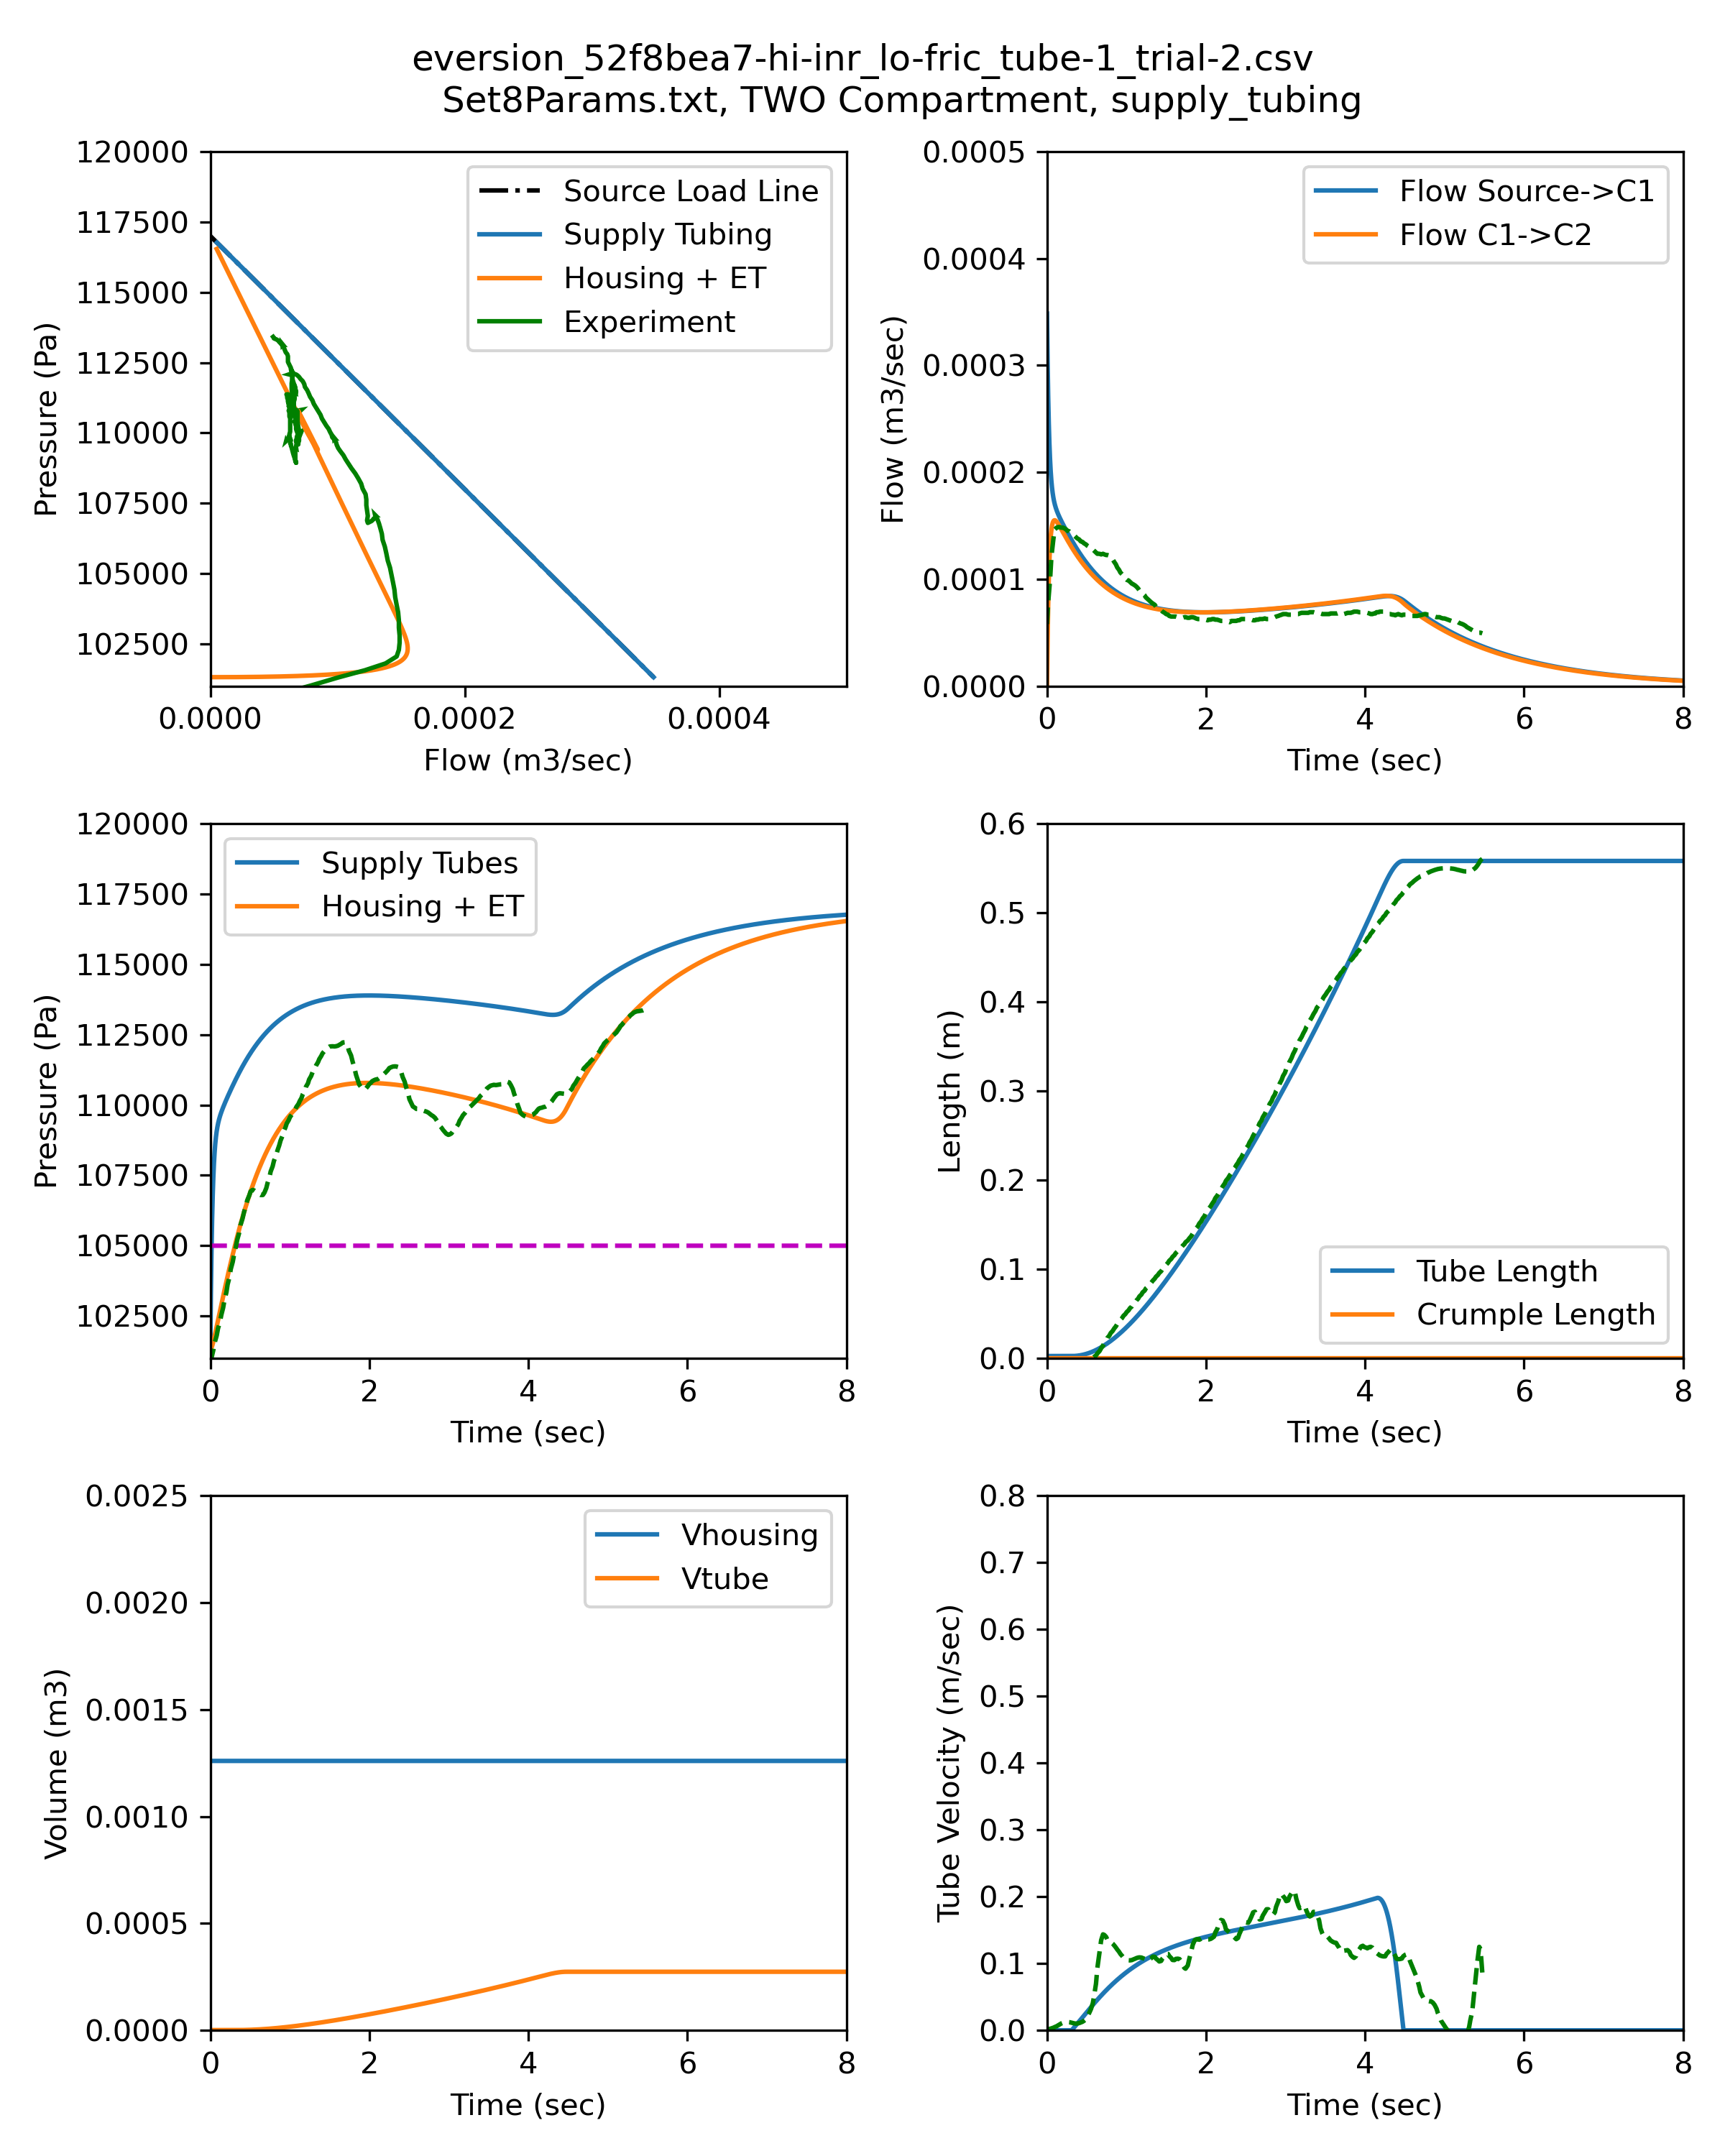
\includegraphics[width=0.475\textwidth]{9Files_Sim_outputs/Set8redo-26-Aug.png}
\caption{Simulation 8.}
\end{figure}


\section{Discussion}

7 of the 10 free parameters were adjusted in order to fit the dataset.
The Threshold Taper feature was not used/needed.
We can measure the magnitude of this adjustment by computing standard devation of
each row of Table \ref{???} (Table \ref{parStd}).
The Pressure Thresholds (PBA\_static and PHalt\_dyn) had small standard deviations
but since they are absolute pressures the variation was larger when compared
to atmospheric pressure (17,280 Pascals) (34\% and 8\% respectively).
Also note that for some eversions, i.e. those with continuous eversion,
PHalt\_dyn was unobservable.

The two drag parameters   Kdrag and K2drag model viscous and length-dependent visousity properties
of the tubing material dragged inside the eversted tubing.  Because of wrinkles,
hardening or softening from repeated cycles, and unknown factors, their high variation
is not surprising. In parameter tuning, they could be used to tune the speed of
eversion, either in continuous eversion, or during the bursts of intermittent eversion.
The K2drag term affected changes in drag at longer lengths and thus can take a
negative value when faster eversion is observed at longer lengths.

\begin{table}\centering
\begin{tabular}{l|l|l}
Parameter       & Mean       & Standard Deviation  (percent) \\\hline
K2drag          & 2.7284E+00 & +/- 5.0648E+00   (185.6\%)  \\
Kdrag           & 2.9346E+00 & +/- 2.5893E+00   (88.2\%)  \\
PBA\_static      & 1.0983E+05 & +/- 5.8829E+03 (5.4\%)  \\
PHalt\_dyn       & 1.0667E+05 & +/- 1.0260E+04  (9.6\%)  \\
Psource\_SIu     & 1.2772E+05 & +/- 1.3749E+04  (10.8\%)  \\
Rsource\_SIu     & 1.3611E+08 & +/- 3.5806E+07  (26.3\%)  \\
Tau\_coulomb     & 1.9432E-03 & +/- 1.3194E-03  (67.9\%)  \\
Threshold Taper  & 0.0000E+00 & +/- 0.0000E+00  (0.0\%)\\
\end{tabular}\label{parStd}
\caption{Variation in parameter values required to achieve realistic simulations.}
\end{table}

\end{document}
